\documentclass[11pt,a4paper]{article}

\usepackage{amsmath,amssymb,amsthm}
\usepackage{enumitem}
\usepackage{geometry}
\usepackage{hyperref}
\usepackage{xcolor}
\usepackage{float}
\usepackage{subcaption}
\usepackage{mdframed}
\usepackage{booktabs}
\usepackage{array}
\usepackage{tcolorbox}
\tcbuselibrary{skins, breakable}

\geometry{margin=1in}

% ── solution environment ─────────────────────────────────────────────────────
\newenvironment{solution}{%
    \begin{tcolorbox}[
        breakable,
        colback=green!4,
        colframe=green!50!black,
        fonttitle=\bfseries,
        title={Model Solution},
        left=6pt, right=6pt, top=4pt, bottom=4pt
    ]%
    }{%
    \end{tcolorbox}%
}

% ── marks command ────────────────────────────────────────────────────────────
\newcommand{\mks}[1]{\hfill\textcolor{gray}{\textbf{[#1 marks]}}}

% ── FOL shortcuts ────────────────────────────────────────────────────────────
\newcommand{\fall}[1]{\forall #1\,}
\newcommand{\fex}[1]{\exists #1\,}

\usepackage{biblatex}
\addbibresource{seqan2.bib}

\title{Sequenzanalyse 2 - Abgabe 2}
\author{Laura Häger und Liliana Sanfilippo}

\begin{document}

    \maketitle

    \section{Aufgabe 1}
    \subsection{Wir arbeiten in dieser Aufgabe mit den Reads in /prj/seqan/Assembly/reads.fq, die im fastq-
    Format vorliegen}
    \paragraph{Informiere dich über dieses Format}
    Okay.
    \paragraph{Erkläre kurz die Unterschiede zum fasta-Format} Das fastq-Format basiert auf dem fasta-Format. Es beinhaltet mehr Informationen über die Sequenz. Diese Informationen werden durch weitere Zeilen dargestellt, so dass jede Sequenz vier Zeilen hat, statt nur eine wie in einer fasta-Datei. Die vier Zeilen sind einmal die Indentifizierungszeile, die Sequenz selbst, die Indentifizierungszeile mit einem Plus davor und ein Qualitäts-Score für jede Base bzw. Position der Sequenz (\textit{associated per base quality score}). \cite{Cock2010, compgenomr}

    \subsection{Wir werden nun (compacted bi-directed) De Bruijn (Sub-) Graphen für k = 11, 15, 17, 21, 31 mit
    ggcat erzeugen. Um diese Graphen später mit Bandage visualisieren zu können, brauchen wir sie im GFA-Format}
    Gemacht mit:
    \begin{verbatim}
ggcat build --gfa-v1 --kmer-length 11 reads.fq -o output11.gfa

ggcat build --gfa-v1 --kmer-length 15 reads.fq -o output15.gfa

ggcat build --gfa-v1 --kmer-length 17 reads.fq -o output17.gfa

ggcat build --gfa-v1 --kmer-length 21 reads.fq -o output21.gfa

ggcat build --gfa-v1 --kmer-length 31 reads.fq -o output31.gfa
    \end{verbatim}

    \paragraph{Schaue dir außerdem die Kommandozeilenparameter -e und -s an.}
    -e ist ein Output-Modus und wird benutzt für ``build links between maximal unitigs'', also es erstellt die Kanten zwischen allen Knoten. -s setzt die ``Minimum multiplicity required to keep a kmer'', also wie oft ein kmer auftauchen muss, damit es einbezogen wird.  \cite{ggcat}

    \paragraph{Wie musst du sie setzen, um einen De Bruijn Graphen mit Kanten und von allen in den Reads enthaltenen k-meren zu erzeugen?}
    Für -s muss man als -s 1 verwenden, damit jedes kmer behalten/verwendet wird und -e kann man einfach so benutzen, da --generate-maximal-unitigs-links der default ist und wir genau das wollen.

    \noindent Gemacht in der Art:
    \begin{verbatim}
ggcat build --gfa-v1 --kmer-length 11 -s 1 -e reads.fq -o output11.gfa
.
.
.
    \end{verbatim}

    \subsection{Visualisiere die erzielten Ergebnisse mit Bandage und bilde sie in deiner Abgabe ab}
    \begin{figure}[H]
        \centering
        \begin{subfigure}[t]{0.3\textwidth}
            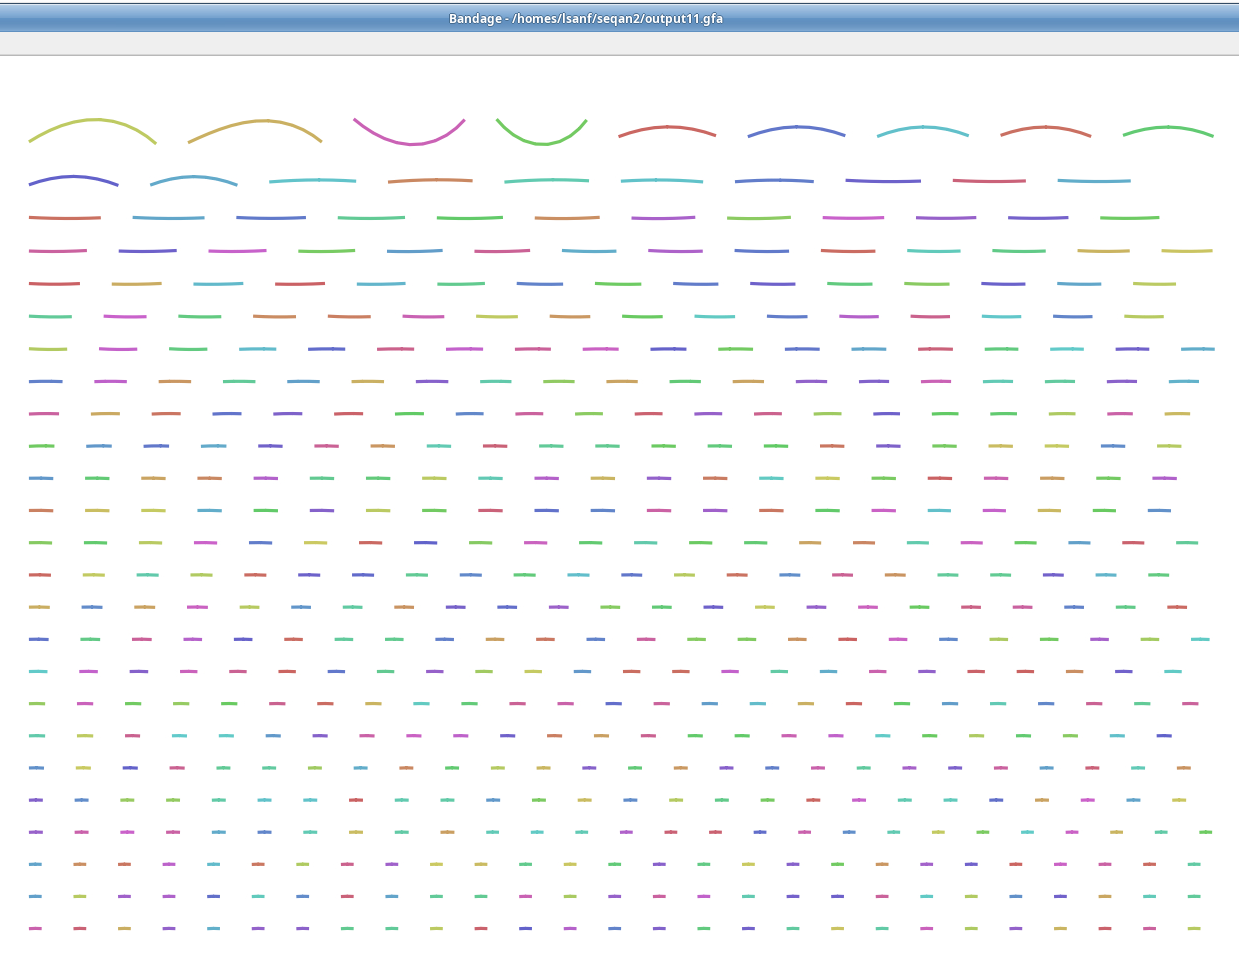
\includegraphics[width=\linewidth]{gfa11.png}
            \caption{Mit k=11}
        \end{subfigure}
        \hfill
        \begin{subfigure}[t]{0.3\textwidth}
            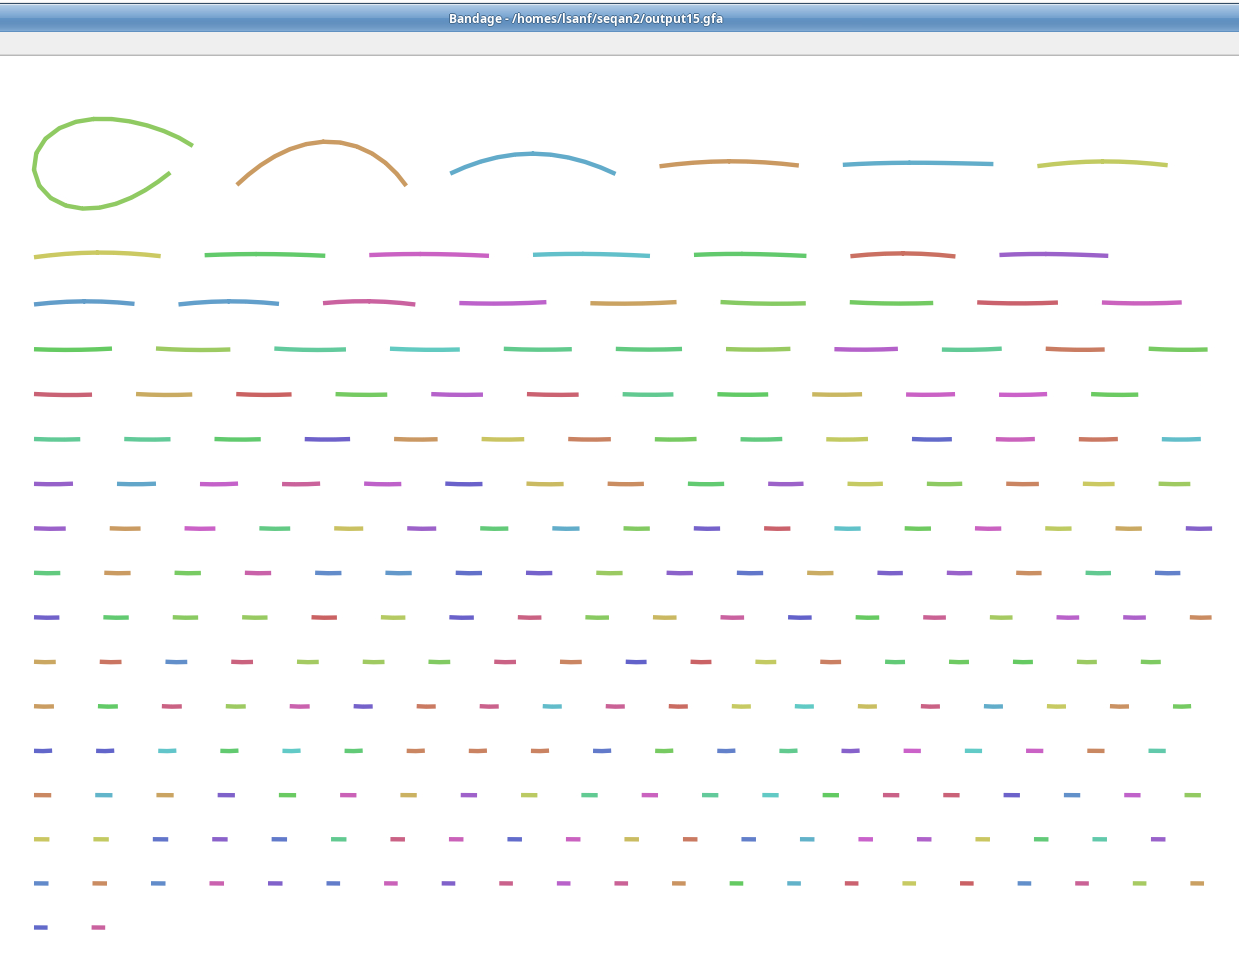
\includegraphics[width=\linewidth]{gfa15.png}
            \caption{Mit k=15}
        \end{subfigure}
        \hfill
        \begin{subfigure}[t]{0.3\textwidth}
            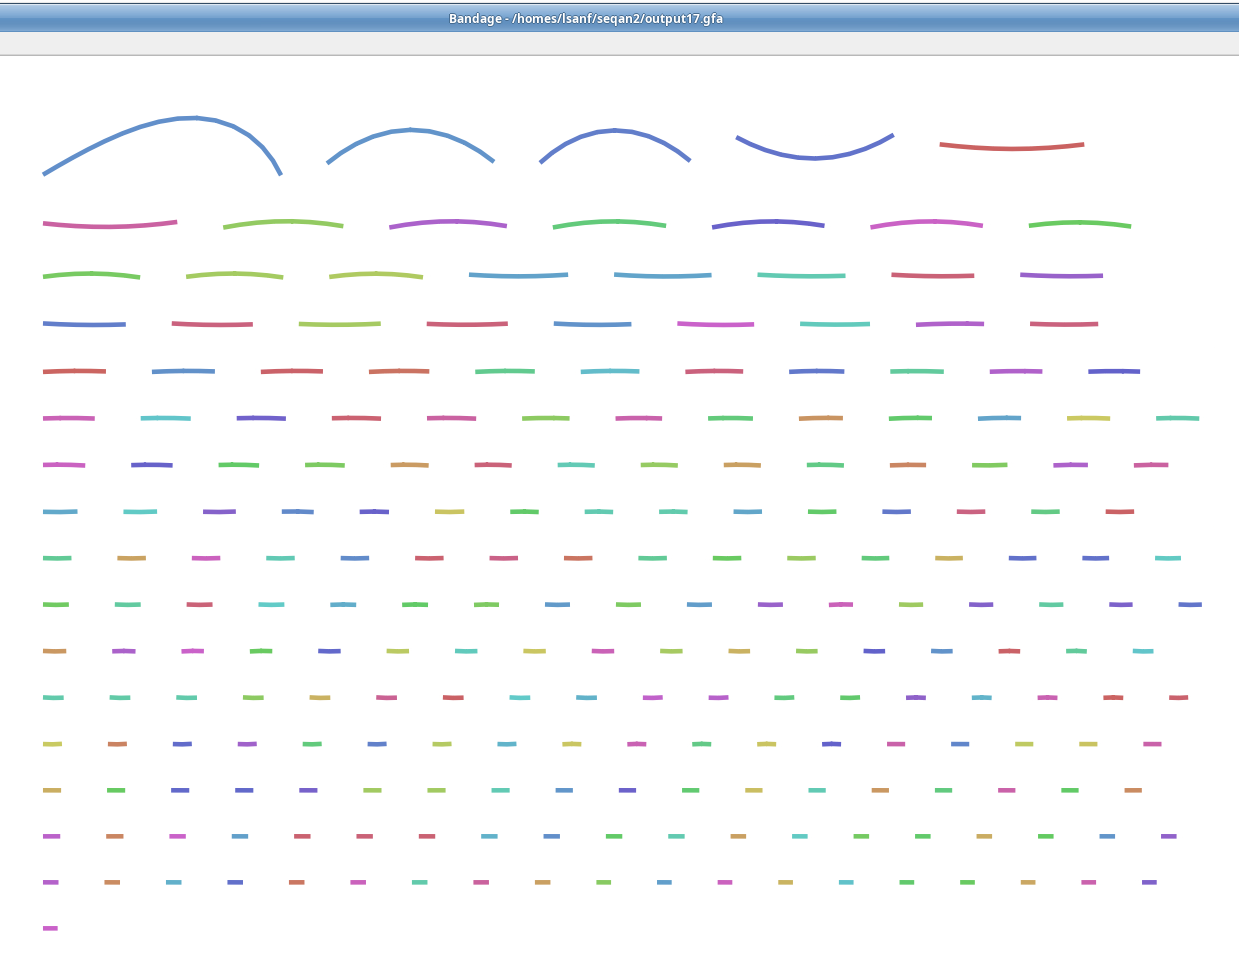
\includegraphics[width=\linewidth]{gfa17.png}
            \caption{Mit k=17}
        \end{subfigure}
        \hfill
        \begin{subfigure}[t]{0.3\textwidth}
            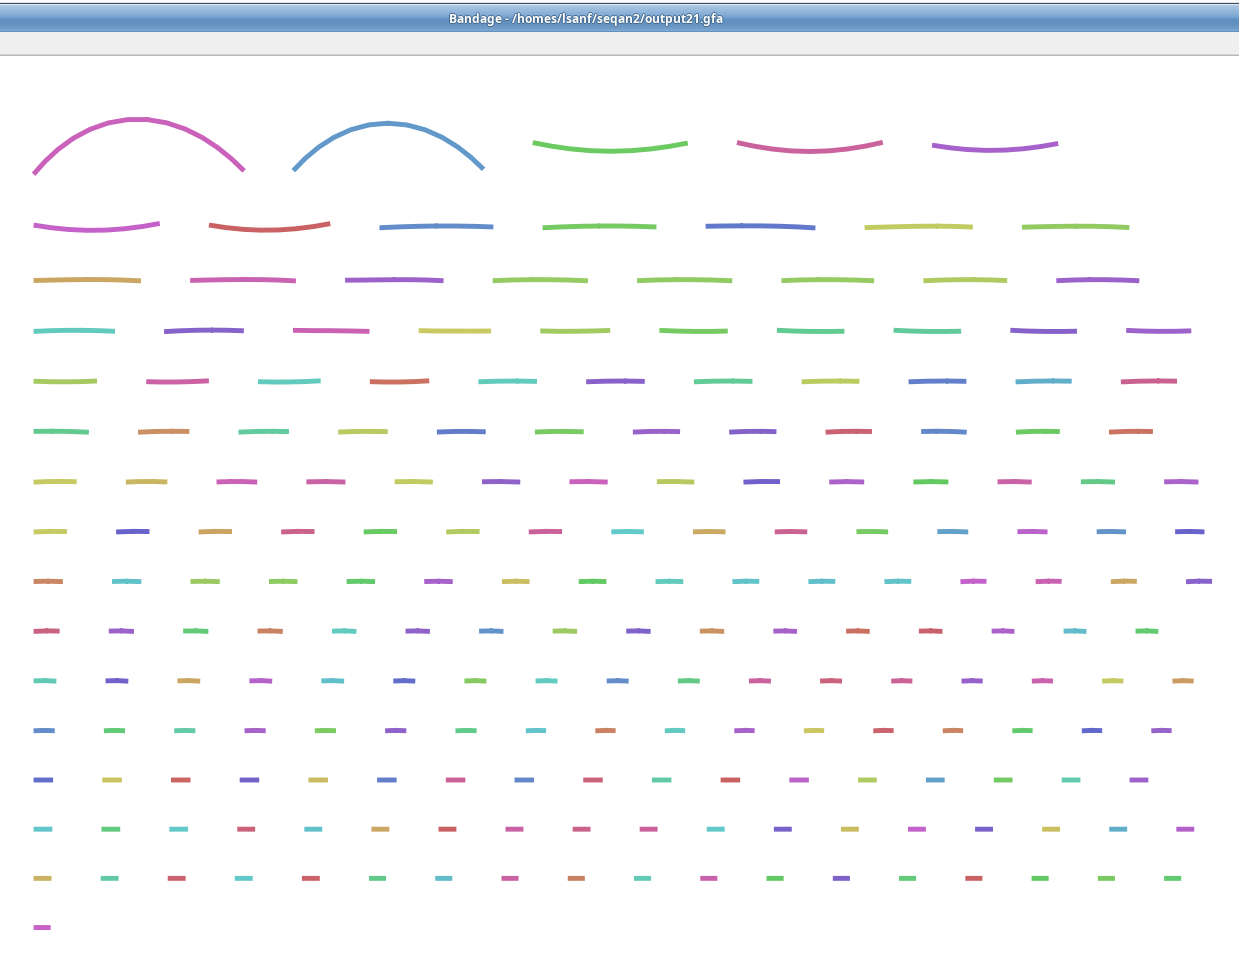
\includegraphics[width=\linewidth]{gfa21.png}
            \caption{Mit k=21}
        \end{subfigure}
        \begin{subfigure}[t]{0.3\textwidth}
            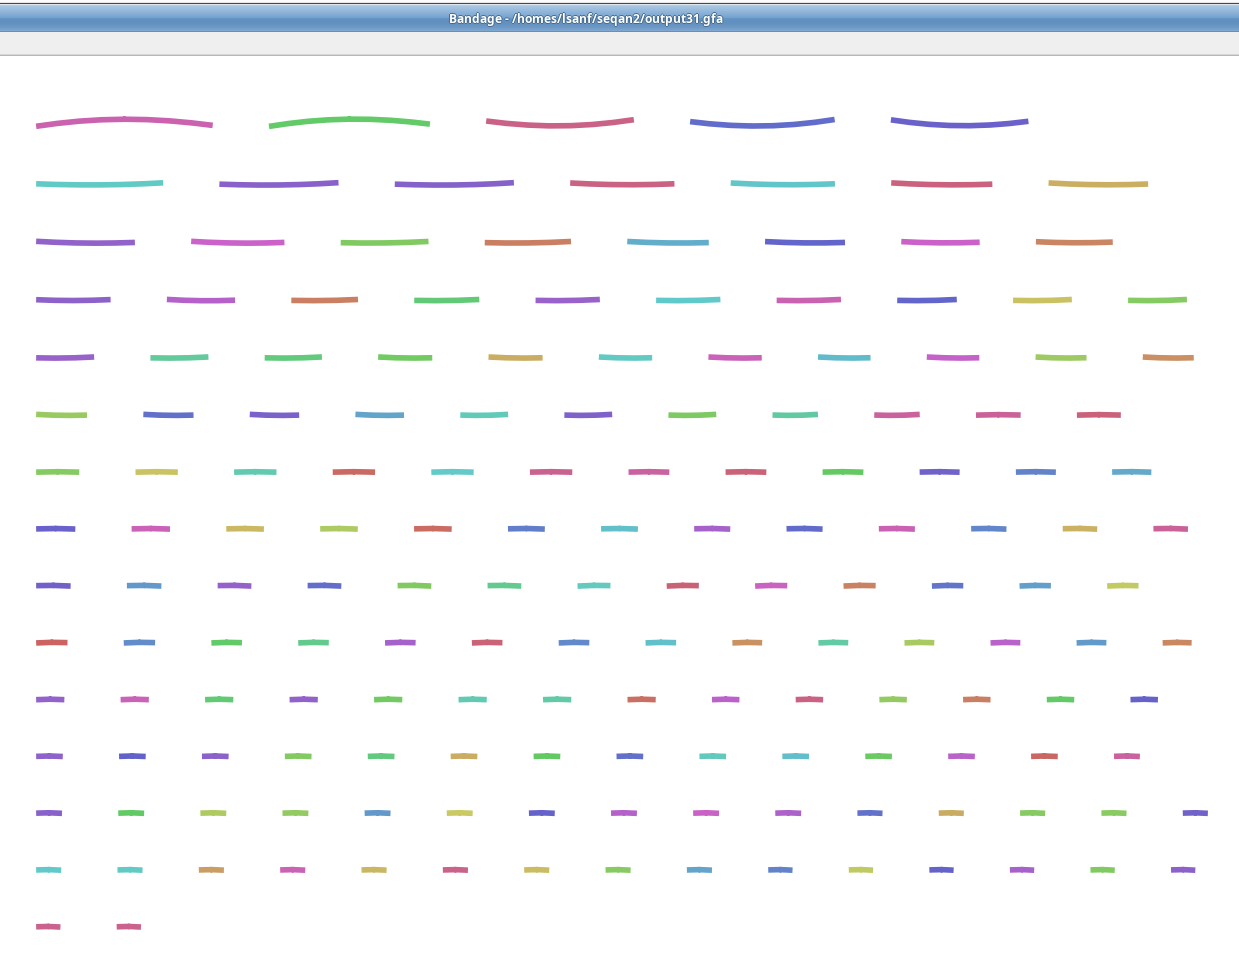
\includegraphics[width=\linewidth]{gfa31.png}
            \caption{Mit k=31}
        \end{subfigure}
        \caption{Hier kann man ganz wunderbar sehen, was passiert, wenn man "-s 1 -e" nicht anwendet.}
    \end{figure}
    Nun aber Schluss mit lustig, hier die tatsächlichen Visualisierungen:
    \begin{figure}[H]
        \centering
        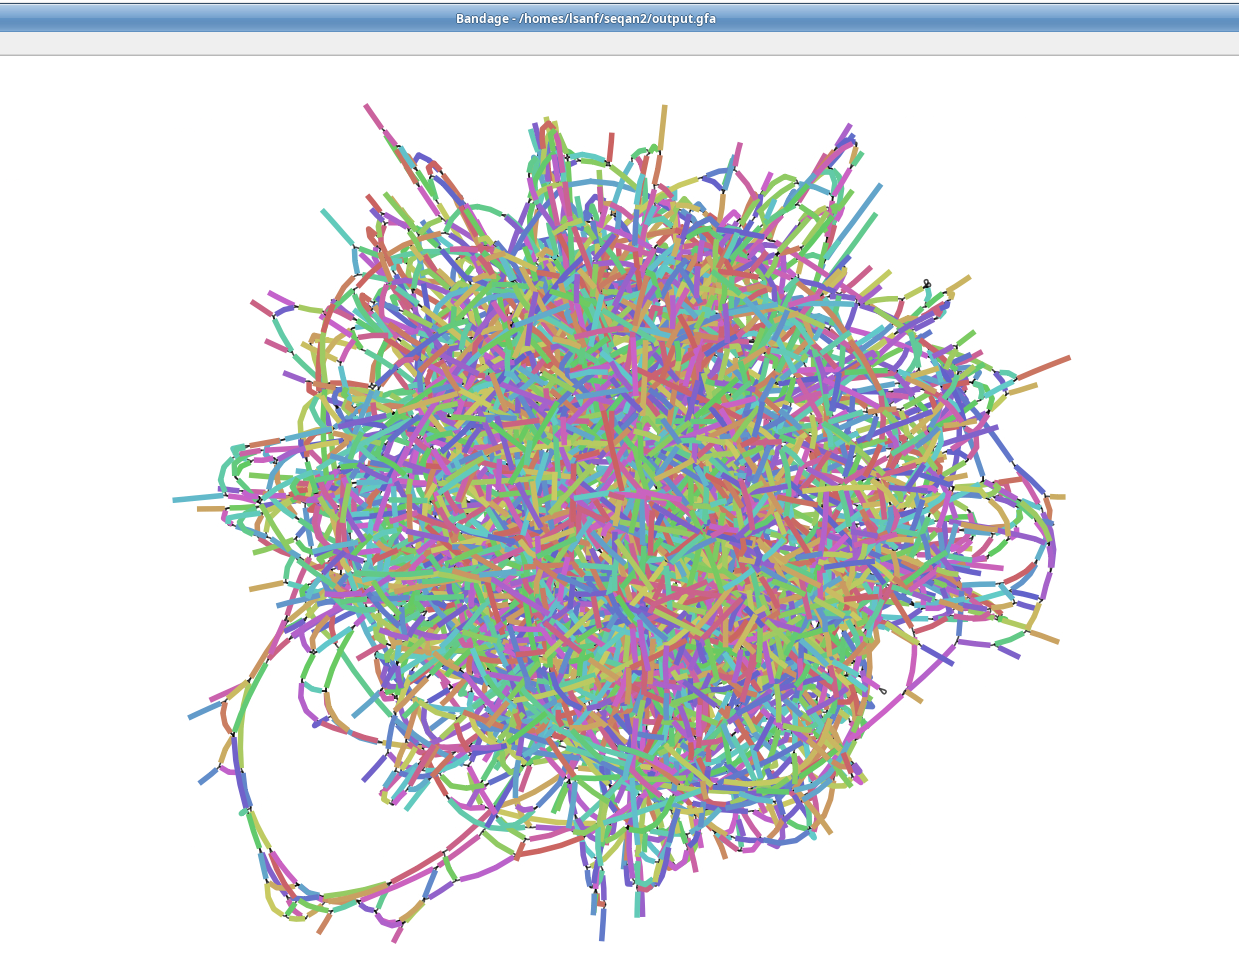
\includegraphics[width=0.5\linewidth]{gfa11se.png}
        \caption{Mit k=11}
    \end{figure}
    \begin{figure}[H]
        \centering
        \begin{subfigure}[t]{0.45\textwidth}
            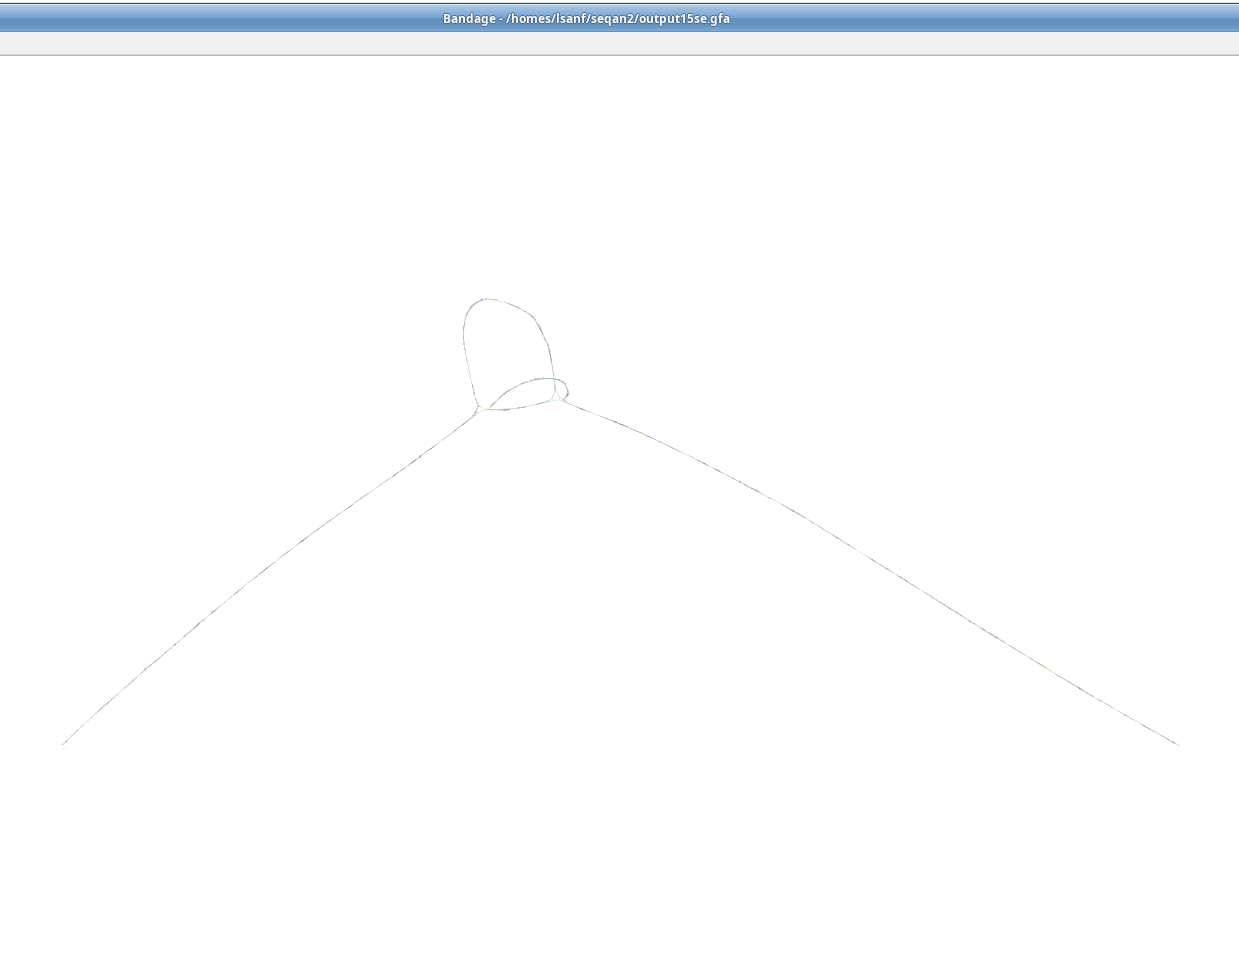
\includegraphics[width=\linewidth]{gfa15se.png}
            \caption{Übersicht}
        \end{subfigure}
        \hfill
        \begin{subfigure}[t]{0.45\textwidth}
            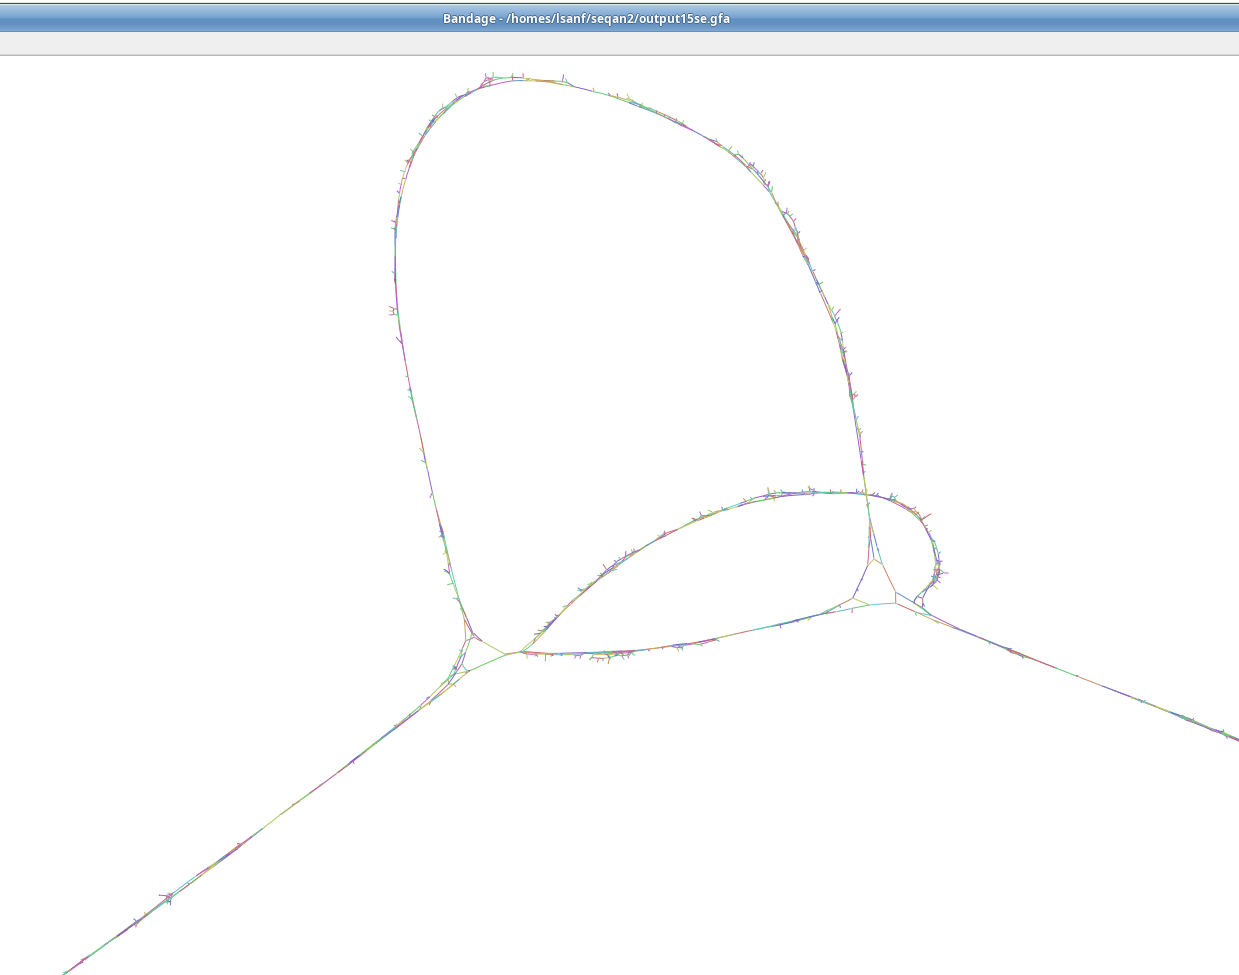
\includegraphics[width=\linewidth]{gfa15se_20.png}
            \caption{Zoom ca. 20\%}
        \end{subfigure}
        \caption{Mit k=15}
    \end{figure}

    \begin{figure}[H]
        \centering
        \begin{subfigure}[t]{0.45\textwidth}
            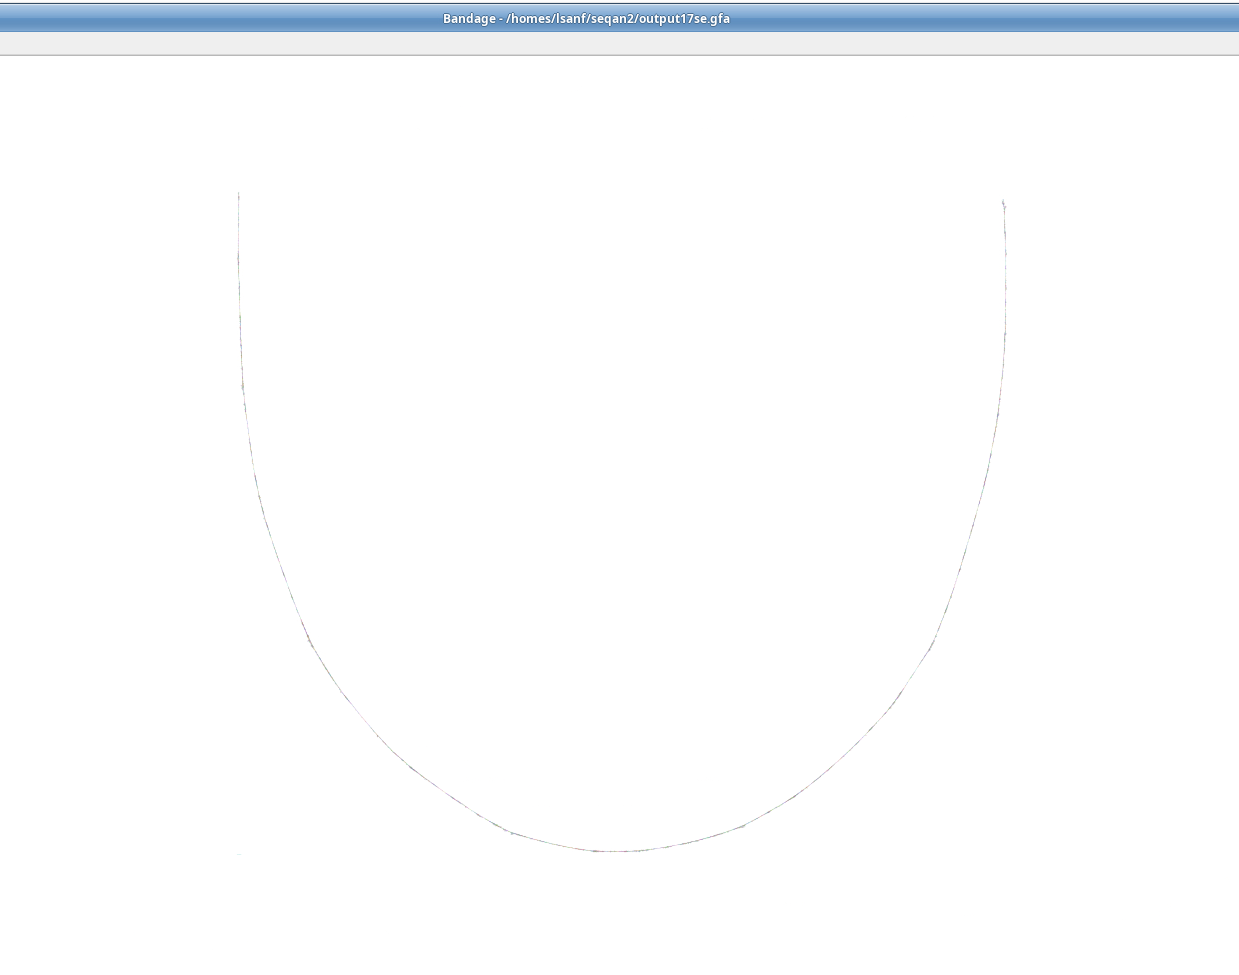
\includegraphics[width=\linewidth]{gfa17se.png}
            \caption{Übersicht}
        \end{subfigure}
        \hfill
        \begin{subfigure}[t]{0.45\textwidth}
            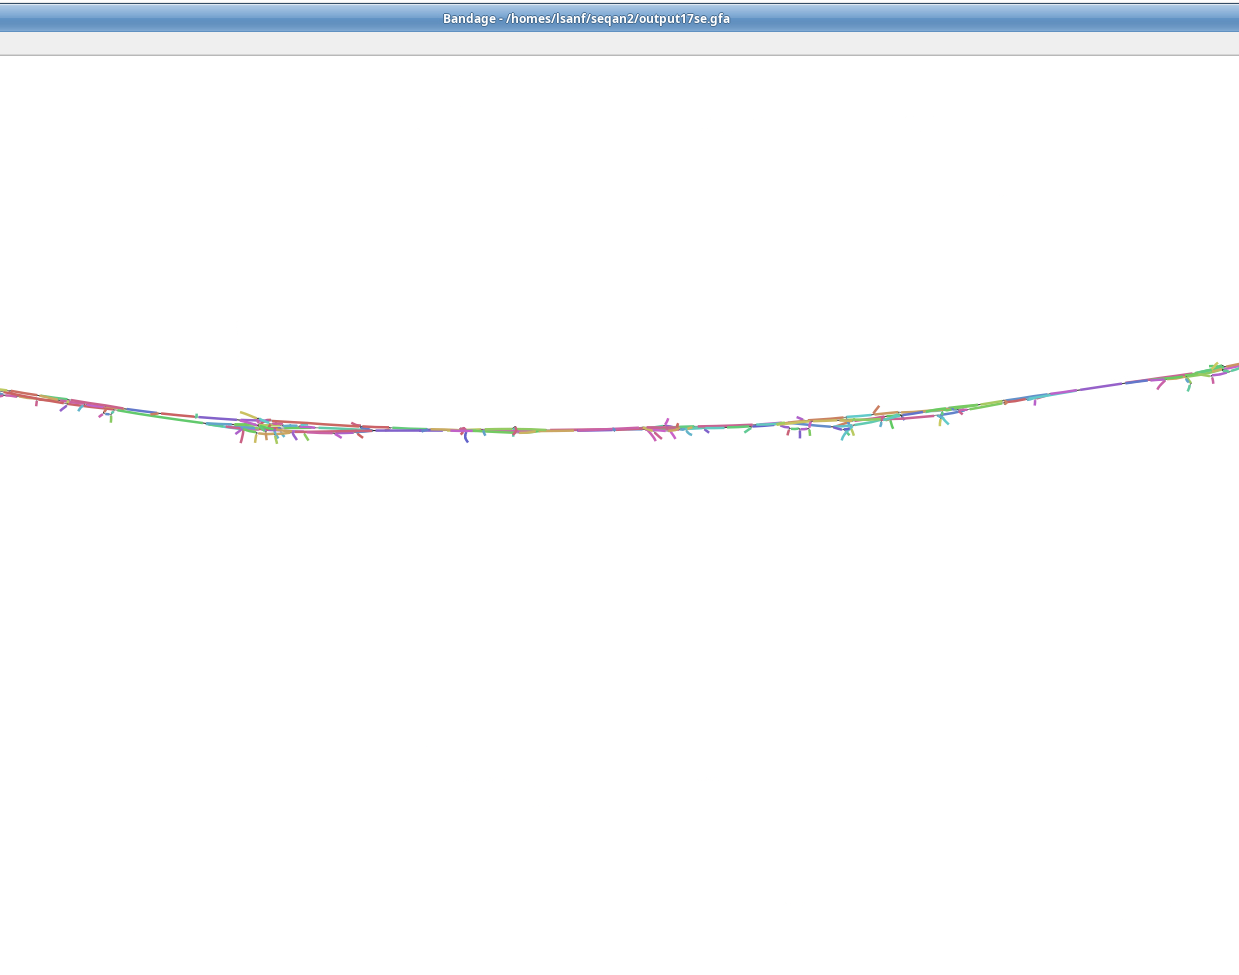
\includegraphics[width=\linewidth]{gfa17se_50.png}
            \caption{Zoom ca. 50\%}
        \end{subfigure}
        \caption{Mit k=17}
    \end{figure}


    \begin{figure}[H]
        \centering
        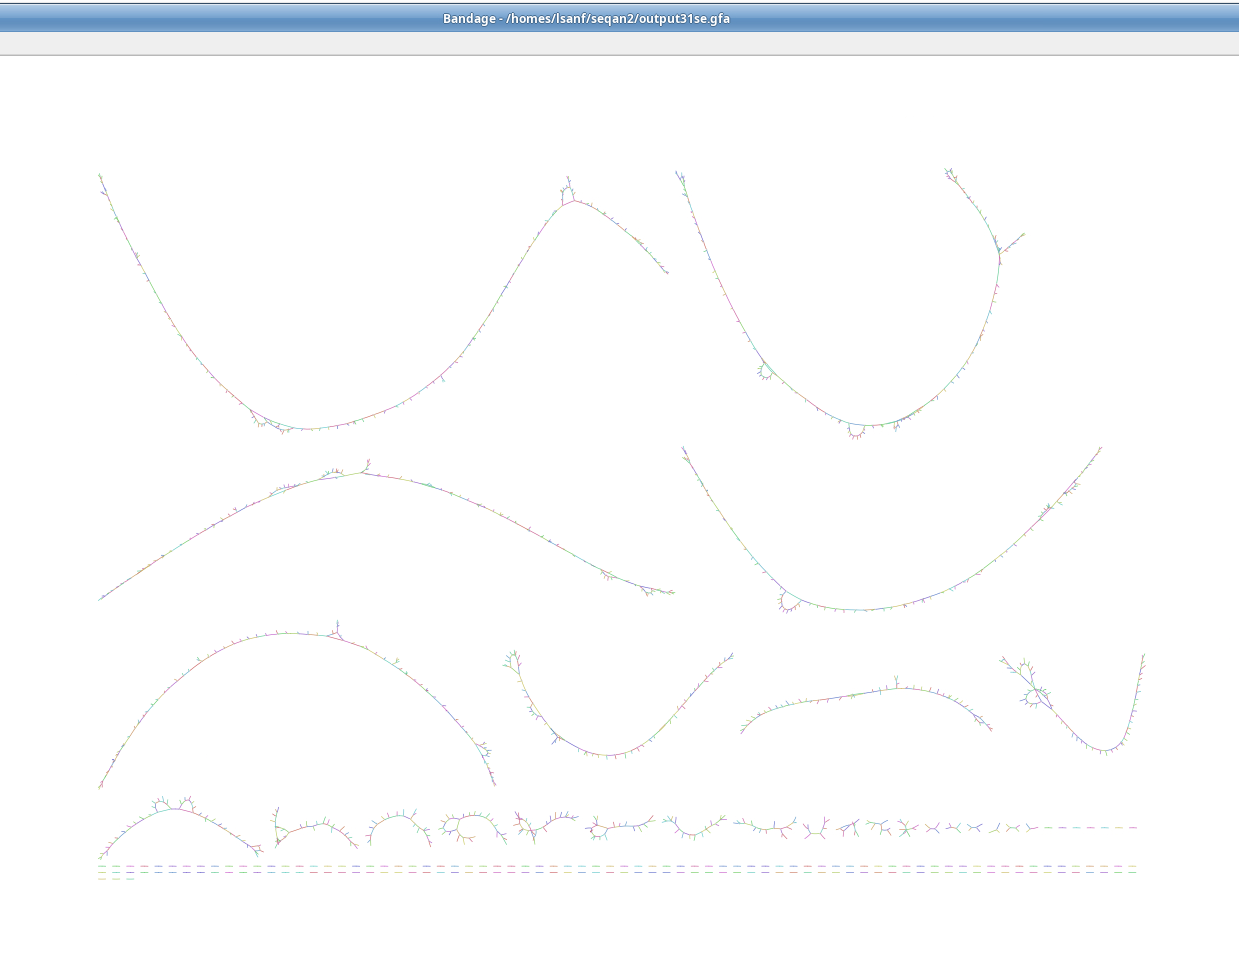
\includegraphics[width=0.65\linewidth]{gfa31se.png}
        \caption{Mit k = 31}
        \label{fig:k31}
    \end{figure}

    \begin{figure}[H]
        \centering
        \begin{subfigure}[t]{0.45\textwidth}
            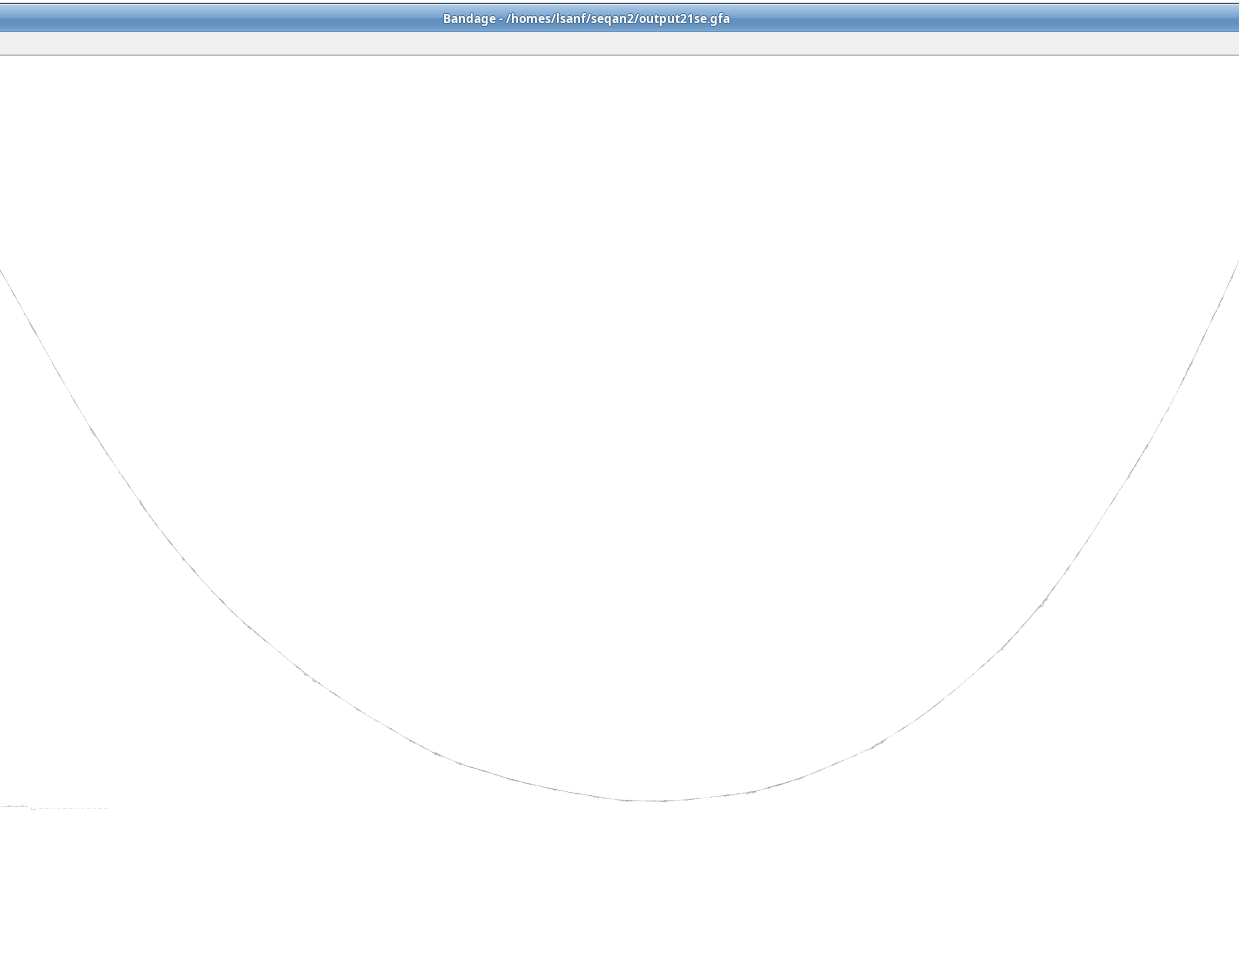
\includegraphics[width=\linewidth]{gfa21se.png}
            \caption{Übersicht}
        \end{subfigure}
        \hfill
        \begin{subfigure}[t]{0.45\textwidth}
            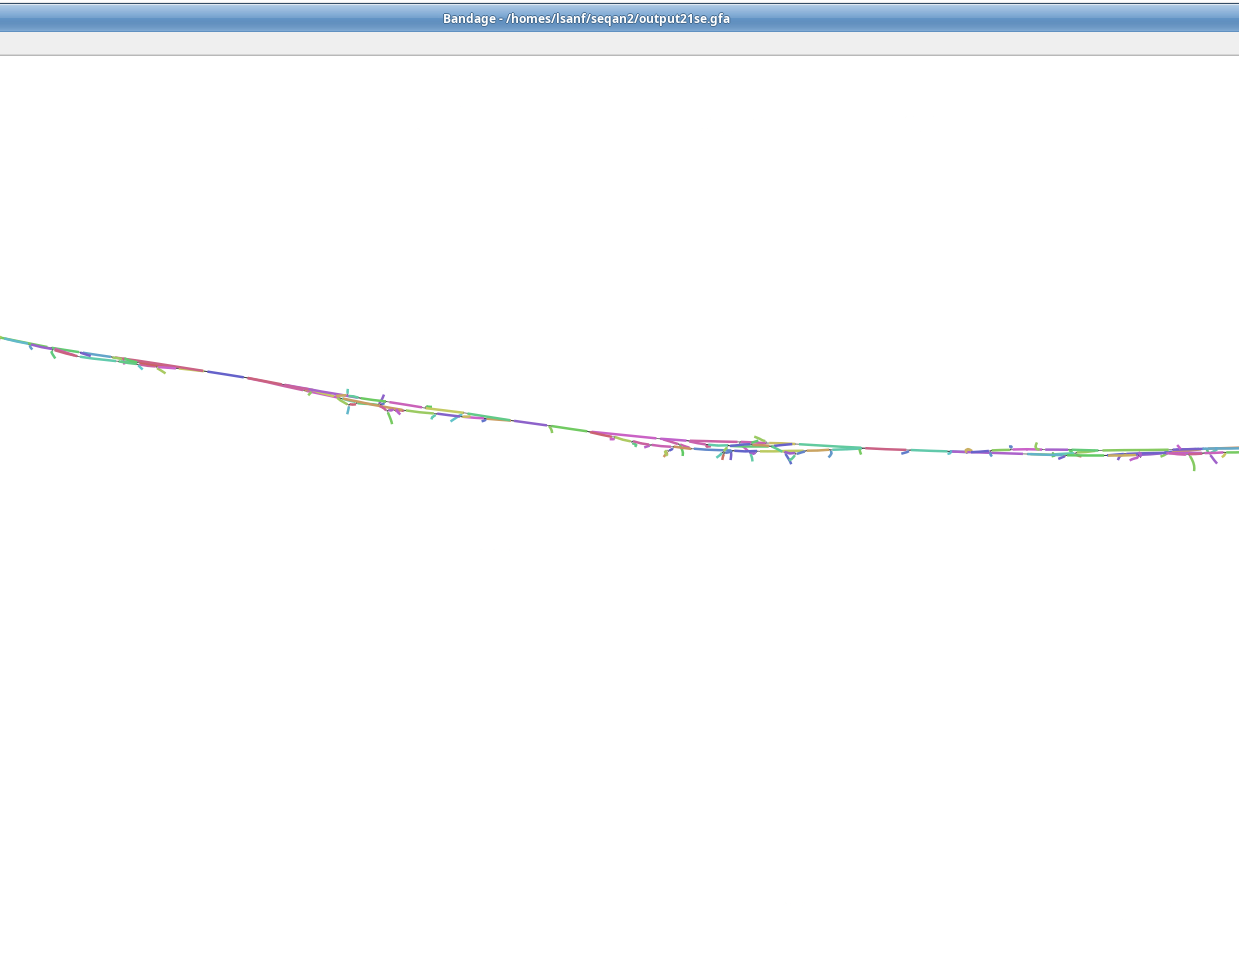
\includegraphics[width=\linewidth]{gfa21se_50.png}
            \caption{Zoom ca. 50\%}
        \end{subfigure}
        \begin{subfigure}[t]{0.45\textwidth}
            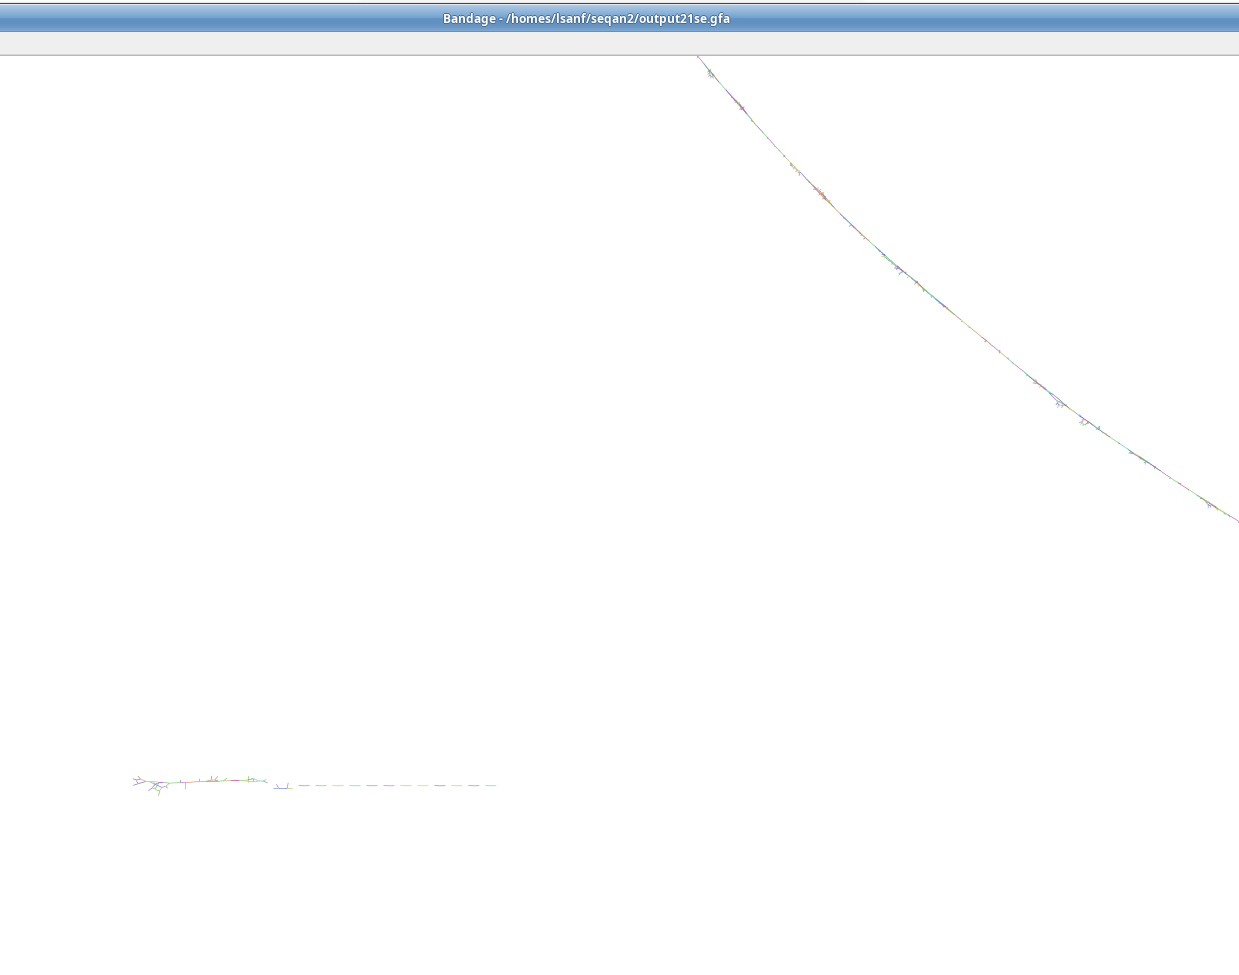
\includegraphics[width=\linewidth]{gfa21se_15.png}
            \caption{Herausstellung des unverbundenen Teils, Zoom ca. 15\%}
            \label{fig:k21zoom15}
        \end{subfigure}
        \caption{Mit k=21}
    \end{figure}

    \paragraph{Wie unterscheiden sich die erzeugten Graphen?}
    Je kleiner das k ist, desto verzweigter, aber auch kompakter, ist der Graph und desto mehr Kanten gibt es insgesamt. Die Verzweigungen sind bilden auch kleinere Schleifen bei kleinen k.

    Bei größeren k ist der Graph nicht mehr vollständig zusammenhängend.
    \paragraph{Erkläre kurz in Bezug auf k wie die Unterschiede zustandekommen.}
    Bei kleineren ks sind die k-mere kürzer und daher kommen sie öfter vor und es müssen viele Kanten zwischen den Knoten gebildet werden. Daher sind die Graphen kompakt, aber unübersichtlich. Es ist sozusagen alles recht nah aneinander, aber auch nicht sonderlich aussagekräftig.

    Wählt man größere k, so werden die Schleifen und Verzweigungen (visuell) größer, da es weniger Verbindungen zwischen k-meren gibt und nicht mehr alles ein Knäuel ist, sondern sich die tatsächlichen Sequenzen besser herauskristallisieren.

    Ab einer bestimmten Größe (hier bereits ab k=21) ist der Graph nicht mehr unbedingt zusammenhängend. Das liegt daran, dass aufgrund von Fehlern in den Daten sich nicht alle k-mere mit (min. 2) anderen überlappen und so ist es nicht möglich eine einzige, fortlaufende Sequenz zu rekonstruieren.


    \subsection{Viele Assembler basieren auf de Bruijn Graphen. Einer von ihnen ist velvet. Lies dir das zugehörige Paper1 durch und beantworte folgende Fragen:}
    \paragraph{Wie unterscheidet sich der Velvet-Graph von einem gewöhnlichen De Bruijn (Sub-) Graphen?}
    Velvet benutzt bidirektionale, kompakte De Bruijn (Sub-)Graphen.

    \paragraph{Wie beeinflusst die Wahl der k-mer-Länge das Ergebnis des Assemblys?}
    Die Wahl der k-mer Länge beeinflusst den Aufbau des Graphen. Dabei sorgt eine kleinere k-mer-Länge dafür, dass mehr Knoten vorliegen, mehr Überlappungen gefunden werden und der Graph somit mehr Kanten hat. Wenn generell mehr Überlappungen gefunden werden, steigt jedoch zwangsläufig die Anzahl irrtümlich identifizierter Überlappungen und damit sinkt die Spezifität des Assemblies und es kann zu Fehlern in der Rekonstruktion der Sequenz kommen.

    Eine größere k-mer Länge reduziert die Anzahl an Knoten und es werden weniger Überlappungen gefunden. Bei großen k-mer-Längen und niedriger Abdeckung kann es im ungünstigsten Fall zu zusammenhangslosen, und somit nutzlosen, Graphen kommen. Bei weniger Überlappungen steigt jedoch die Spezifität und irrtümlich identifizierte Überlappungen werden unwahrscheinlicher.

    Je nach Abdeckung muss entschieden werden, ob die Spezifität (lange k-mere) oder die Sensitivität gegenüber Überlappungen (kurze k-mere) priorisiert werden soll. Außerdem muss die k-mer Länge ungerade sein, damit ein k-mer nicht sein eigenes reverses Komplement sein kann und echt kleiner als die Read-Länge, damit überlappungen gefunden werden können. Es kann jedoch auch bereits bei echt kleineren k-mer-Längen der Fall sein, dass keine Überlappungen mehr gefunden werden können:

    \paragraph{Kann für k eine gerade Zahl gewählt werden? Warum?/Warum nicht?}
    Nein, man muss eine ungerade Zahl wählen, damit k nicht sein eigenes reverses Komplement sein kann. ("To ensure
    that each k-mer cannot be its own reverse complement, k must be
    odd.", S. 822)

    \paragraph{Tips und Bubbles sind zwei häufig beobachtete Strukturen in De Bruijn (Sub-) Graphen und
    verwandten Graphen. Finde je ein Beispiel dieser Strukturen in einer der Visualisierungen mit
    Bandage und bilde sie in deiner Abgabe ab.}
    Im Paper steht zu Tips: "A tip is a chain of nodes that is disconnected on one end." Das ist bspw. in Abbildung \ref{fig:k31} (mehrfach) und \ref{fig:k21zoom15} zu sehen.

    Bubbles bestehen aus zwei Pfaden mit ähnlichen Sequenzen, die in den selben Knoten beginnen und enden. Man kann davon ausgehen, dass sie aufgrund von fehlerhaften Daten entstanden sind und somit redundant.
    \begin{figure}[H]
        \centering
        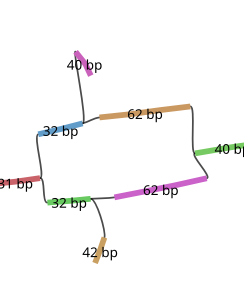
\includegraphics[width=0.4\linewidth]{bubble.png}
        \caption{Mögliche Bubble.}
        \label{fig:bubble}
    \end{figure}

    In Abbildung \ref{fig:bubble} ist eine mögliche Bubble aus dem Graph für k=31 zu sehen. Ohne die Annotation der Sequenzen ist es nicht eindeutig zu sagen, aber da die Längenverteilung sehr ähnlich ist, kann man dies als Beispiel nehmen.

    \paragraph{Beschreibe kurz, wie Velvet mit Tips und Bubbles umgeht.}
    Bubbles werden mit dem sog. Tour-Bus-Algorithmus entfernt, wenn sie als fehlerhaft bzw. redundant befunden wurden. Dies wird auf Basis der Sequenzidentität und Länge bestimmt.

    Wenn Tips als fehlerhaft eingestuft werden, weil zu vermuten ist, dass schlichtweg eine Lücke in der Abdeckung ist, dann werden sie nicht entfernt. Ansonsten werden sie einfach entfernt.

    Tips sind fehlerhaft, wenn sie kürzer als 2000bp sind oder sie nur eine Alternative zu häufigeren Pfaden sind.

    \subsection{Informiere dich im Manual (z.B. zu finden unter /vol/biotools/share/velvet/) darüber, was die
    Aufgaben von velveth und velvetg sind und nenne sie in deiner Abgabe. Mache dich außerdem
    mit der einfachen Syntax der beiden Programme bekannt.}
    Velvet ist ein aus zwei Programmteilen bestehender Algorithmus für ”de novo” Sequence Assembly und wird über Eingaben in der Kommandozeile genutzt. Der zuerst angewendete Teil namens velveth dient dazu, die zugeführten Sequenz-Daten aufzubereiten, damit sie anschließend durch den zweiten Programmteil velvetg verwendet werden können. Dies geschieht durch die Erstellung von Hash-Tabellen aus den Sequenz-Daten und darauf basierend automatisch erstellten Output-Dateien, die die Sequenzen und eine Roadmap enthalten.

    Durch einen Aufruf des zweiten Teilprogramms velvetg werden aus den vorbereiteten Daten de Bruijn-Graphen erstellt und diese vereinfacht und korrigiert. Anschließend werden alle Contigs länger als das Zweifache der gesetzten Wortlänge k in einer Datei ausgegeben und weitere Dateien mit Informationen über die Graphen erstellt. In der Anwendung muss darauf geachtet werden, dass der genannte Ausgabeordner mit dem Ordner übereinstimmt, in dem vorher die Output-Dateien von velveth gespeichert wurden.
%Wir haben außerdem den de Bruijn-Graphen dahingehend gefiltert, dass Knoten mit einer Abdeckung kleiner zehn heraus gefiltert wurden, um Fehler in der Assembly zu mindern.


    \subsection{Teste Velvet mit k = 11, 15, 17, 21, 31 auf den Reads. Nutze dazu einen Coverage-Cutoff von 3}

    \paragraph{Gib
    die verwendeten Kommandozeilenbefehle für velvetg und velveth auch in deiner Abgabe an:}
    Durch die Verwendung des folgenden Befehls haben wir die kurzen Reads aus der Datei test reads bezüglich verschiedener k-mer-Länge verarbeiten lassen.
    \begin{center}
        velveth . 11 -fastq -short reads.fq
    \end{center}
    (Mit den verschiedenen Zahlen natürlich)
    \begin{center}
        velvetg . -cov\_cutoff 3
    \end{center}

    \subsection{Vergleiche anschließend die Ergebnisse.}
    \paragraph{Wie viele Knoten haben deine Graphen und wie unterschei-den sich die n50-Werte?}
    Bei großen oder kleinen k sind die n50-Werte niedriger als bei mittleren k und es gibt auch mehr Knoten im Graph (siehe Tabelle).
    \begin{table}[H]
        \centering
        \begin{tabular}{l|lllll}
            k &  11  & 15 & 17 & 21 & 31 \\ \hline
            nodes & 112 & 3 & 1 & 2 & 16\\
            n50 & 107 & 2994 & 5297 & 5046 & 270\\
            max & 312 & 2994 & 5297 & 5046 & 398\\
            total & 5209 & 5298  & 5297 & 6265 & 3336
            % using & 0/1000 & same & same & same
        \end{tabular}
    \end{table}

    \paragraph{Erkläre, wie die Ergebnisse zustande gekommen sind.}
    DFas liegt daran, dass bei kürzeren k-mer-Längen deutlich mehr Überlappungen gefunden werden und dadurch mehr Knoten in den Graphen vorliegen, als bei längeren k-meren. Dass der n50 und die Anzahl der Knoten zusammen hängen ist zu erwarte, da der n50Wert die Qualität des Assemblies beschreibt und große Anzahlen von Knoten auf fehlerhaft identifizierte Überlappungen hinweisen können.

    \subsection{Wähle ein Assembly mit möglichst wenigen Contigs und vergleiche die assemblierte(n) Contig-
    sequenz(en) mit der Referenzsequenz reference.fasta.}
    Dafür nehmen wir die Assembly mit k=17.
    \paragraph{Aligniere die beiden Sequenzen, z.B. mit BLAST}
    Wir haben die BLAST Typ blastn auf der Seite des NCBI genutzt. Query war die Assembly und Subject die gestellte Referenz (siehe Abb. \ref{fig:blast}).
    \begin{figure}[H]
        \centering
        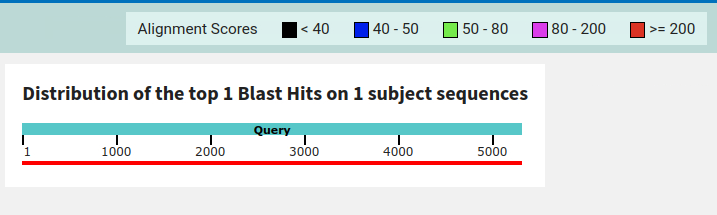
\includegraphics[width=0.7\linewidth]{blast.png}
        \caption{}
        \label{fig:blast}
    \end{figure}

    \paragraph{Diskutiere kurz dein Ergebnis}
    Es gibt 100\%iges Query-Cover und 99.92\% Übereinstimmung Identität, also ist die Assembly komplett in der Referenz enthalten, aber die Referenz ist etwas länger. Die Assembly ist also nicht perfekt, aber nah dran.

    \paragraph{Erstelle einen (compacted bi-directed) De Bruijn (Sub-) Graphen der beiden Sequenzen mit ggcat und visualisiere ihn mit Bandage. Nutze dabei ein eher größeres k.}
    Beide Dateien zusammen in eine kombiniert:
    \begin{center}
        cat reference.fasta k17/contigs.fa $>$ combi.fa
    \end{center}
    Dann mit ggcat erstellt:
    \begin{center}
        ggcat build --gfa-v1 --kmer-length 21 -s 1 -e combi.fa -o out\_combi.gfa
    \end{center}

    \paragraph{Wie sehen die Unterschiede im Graphen aus?}
    Die Unterschiede sind sehr gering.
    \begin{figure}[H]
        \centering
        \begin{subfigure}[t]{0.65\textwidth}
            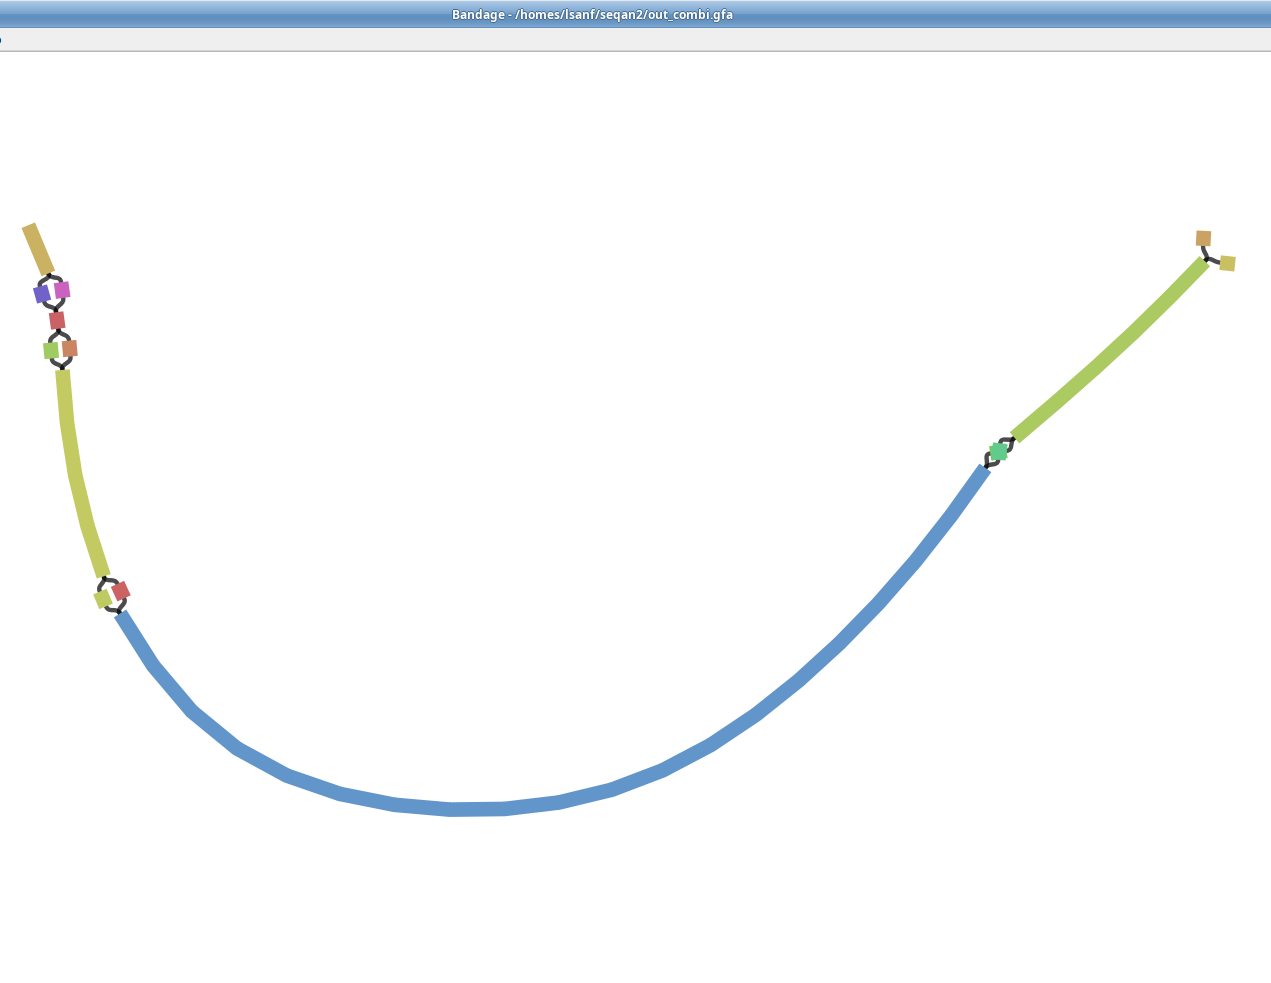
\includegraphics[width=\linewidth]{combi.png}
            \caption{Graph wie von Bandage erstellt.}
            \label{fig:combi}
        \end{subfigure}
        \hfill
        \begin{subfigure}[t]{0.65\textwidth}
            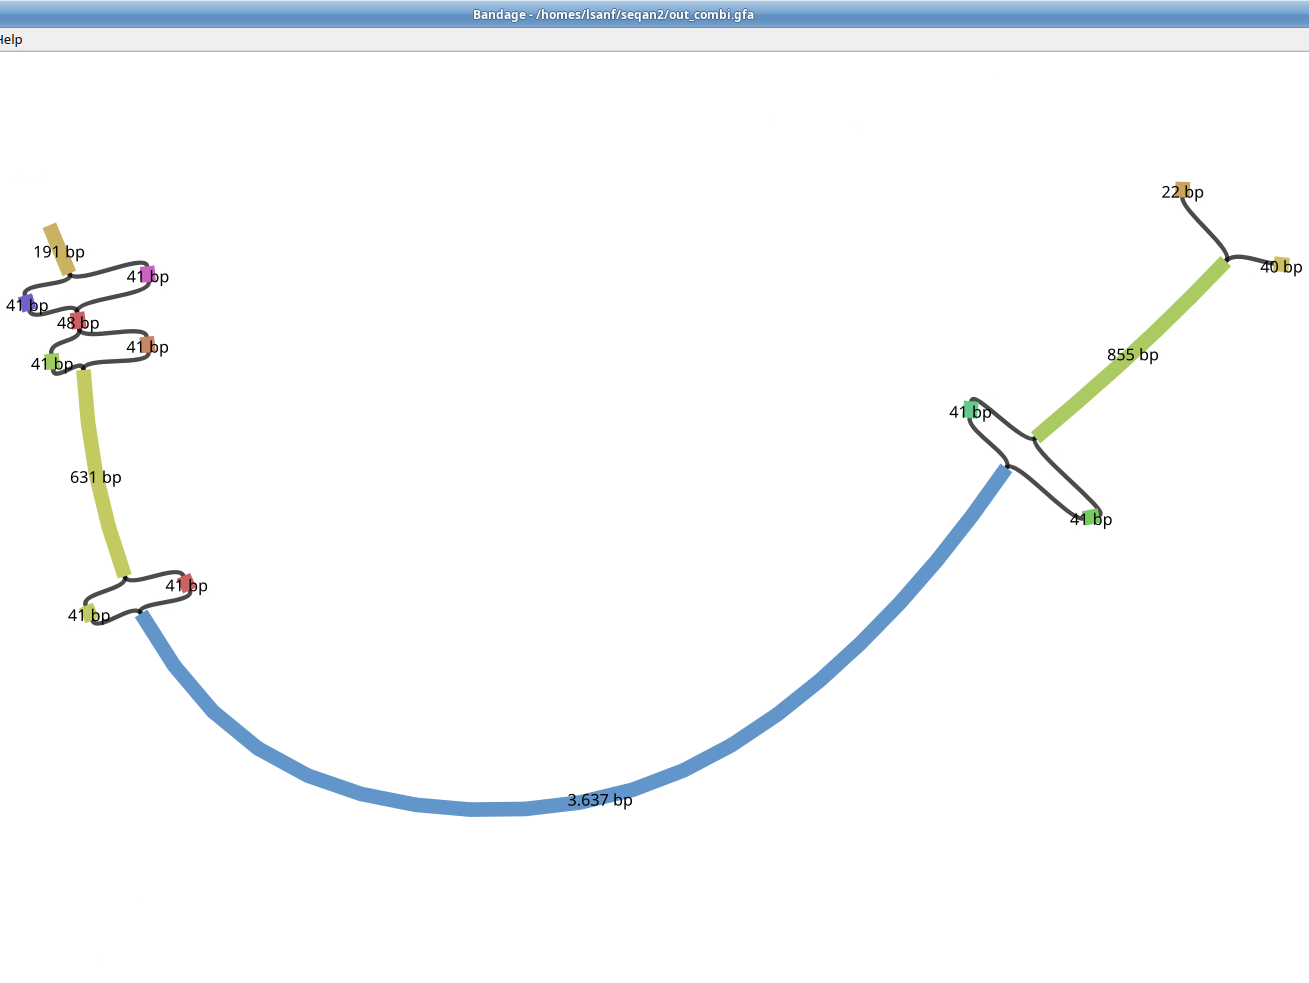
\includegraphics[width=\linewidth]{combi_len.png}
            \caption{Graph mit Annotation der Längen und visuelle entzerrt.}
        \end{subfigure}
        \caption{}
    \end{figure}

    Man kann sehen, dass die Unterschiede an einer begrenzten Anzahl von Stellen ist, über kurze Abschnitte geht und man kann vermuten, dass es sich dabei um Bubbles handelt.

    \printbibliography

\end{document}
